\item A flatcar of mass \( m_0 \) starts moving to the right due to a constant horizontal force \( F \) (Fig: 1.46). Sand spills on the flatcar from a stationary hopper. The velocity of loading is constant and equal to \( \mu \) kg/s. Find the time dependence of the velocity and the acceleration of the flatcar in the process of loading. The friction is negligibly small.
    \begin{center}
        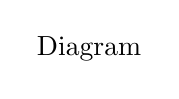
\begin{tikzpicture}
            \node at (0, 0) {Diagram};
        \end{tikzpicture}
    \end{center}
    \begin{enumerate}
        \item This is a subquestion.
        \item This is another subquestion.
    \end{enumerate}
\begin{solution}
    \begin{center}
        \begin{tikzpicture}
            \pic at (0, 0) {frame=3cm};
        \end{tikzpicture}
    \end{center}

    \begin{align*}
        \intertext{Let the car be moving in a reference frame to which the hopper is fixed and at any instant of time, let its mass be \( m \) and velocity \(\vec{v}\).}
        \intertext{Then from the general equation, for variable mass system}
        m\dfrac{d\vec{v}}{dt} &= \vec{F} + \vec{u} \dfrac{dm}{dt} \tag{1.183}\\
        \intertext{We write the equation, for our system as,}
        m\dfrac{d\vec{v}}{dt} &= \vec{F} - \vec{v} \dfrac{dm}{dt} \quad \text{as} \quad \vec{u} = -\vec{v}\\
        \intertext{So,}
        \dfrac{d}{dt}(m\vec{v}) &= \vec{F}\\
        \intertext{and}
        \vec{v} &= \dfrac{Ft}{m} \quad \text{on integration}\\
        \intertext{But}
        m &= m_0 + \mu t\\
        \intertext{so,}
        \vec{v} &= \dfrac{Ft}{m_0 \left( 1 + \dfrac{\mu t}{m_0} \right)}\\
        \intertext{Thus, the sought acceleration is}
        \vec{w} &= \dfrac{d\vec{v}}{dt} = \dfrac{\vec{F}}{m_0 \left( 1 + \dfrac{\mu t}{m_0} \right)^2}
    \end{align*}
\end{solution}
